\chapter{Related Work}

\label{Chapter-Related-Work}

\section{CNN Architectures}
\label{section:CNN-Architectures}
The essential part of every machine learning application is its dataset. A dataset is the collection of data that a machine learning application can be based on; for a neural network application, a dataset is the collection of data that the network is trained and tested. Nowadays, there are numerous datasets for visual recognition applications, with various sizes and qualities. The size of a dataset defines the number of data per class, and its quality can define many aspects of the data, such as their noise characteristics and their factual correctness of assigned labels (the creators of the dataset may wrongly label data). Some of the most popular datasets are MNIST with grayscale images of handwritten digits \cite{The-MNIST-database-of-handwritten-digits} \cite{MNIST-database-Wikipedia}, Fashion-MNIST with grayscale images of various pieces of clothing \cite{Fashion-MNIST-a-Novel-Image-Dataset-for-Benchmarking-Machine-Learning-Algorithms} \cite{Fashion-MNIST-Github}, CIFAR-10 \& CIFAR-100 with color images of 10 and 100 classes, respectively, of everyday items \cite{CIFAR-10-CIFAR-100} \cite{CIFAR-10-CIFAR-100-Wikipedia}, Microsoft COCO with color images for object recognition / detection of everyday items \cite{Microsoft-COCO-Common-Objects-in-Context} \cite{MS-COCO} and ImageNet with high resolution color images of 22000 classes of everyday items \cite{ImageNet-Official-site} \cite{ImageNet-Wikipedia}.

ImageNet is one of the biggest datasets, containing more than 14 million hand-annotated images and more than 1 million bounding boxes for those images. Since 2010, the ImageNet Large Scale Visual Recognition Challenge (ILSVRC) is organized annually by the ImageNet project, where software programs compete in the classification of a trimmed list of one thousand non-overlapping classes. The contestant softwares have been of many different types throughout the years; however, from the ILSVRC 2012 and then on, Convolutional Neural Networks have dominated the challenge, achieving near human-like accuracy. A CNN called AlexNet \cite{ImageNet-classification-with-deep-convolutional-neural-networks} managed to achieve a top-5 error of 15.3\% in the ILSVRC 2012, where the top-5 error rate is the fraction of test data for which the correct label is not among the five most probable labels.

Many CNN architectures have been created using the aforementioned data\-sets. Some of the most important ones are being described below.

\subsection{LeNet-5}
LeNet-5 \cite{Gradient-based-learning-applied-to-document-recognition} (Figure \ref{fig:LeNet-5}), created by LeCun et al in 1998, was, at the time, a pioneering 7-layer convolutional neural network designed to recognize simple 32x32 grayscale digit images, similar to those on the MNIST dataset. It uses two convolutional layers, two pooling layers, and three fully-connected layers. However, it can only support low-resolution images and few classes, due to its low learning capacity. For higher resolution images, deeper networks are required, which was not feasible back then because of limited hardware performance. LeNet-5 was the first success for CNNs.

\begin{figure} [H]
	\centering
	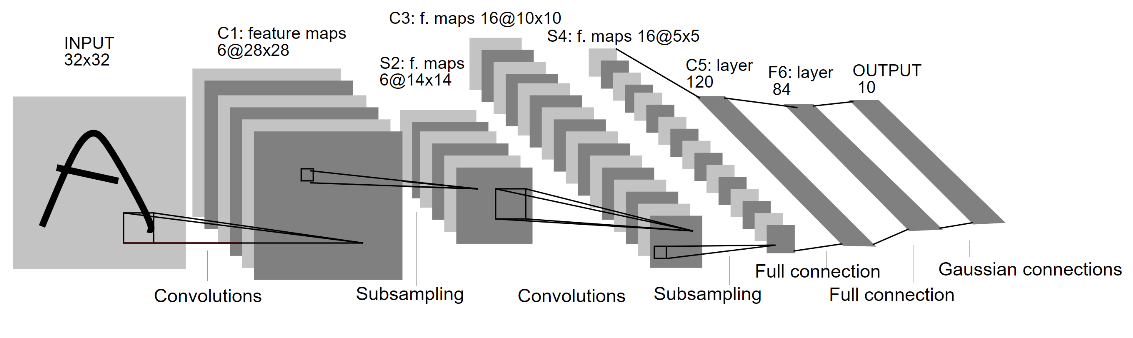
\includegraphics[width=\textwidth]{Images/CNNArchitectures/LeNet-5.png}
	\decoRule
	\caption[LeNet-5 architecture]{LeNet-5 architecture}
	\label{fig:LeNet-5}
\end{figure}

\subsection{AlexNet}
AlexNet \cite{ImageNet-classification-with-deep-convolutional-neural-networks} (Figure \ref{fig:AlexNet}), created by Alex Krizhevsky et al in 2012, outperformed all prior contestants of the ILSVRC by almost twice increase in accuracy, reducing the top-5 error rate from 26.2\% to 15.3\%. It takes as input RGB 224x224 images. This is achieved by using the same types of layers as LeNet-5, but more of them, making it is deeper and with more filters per layer. Using such deep networks was made feasible due to the utilization of GPUs during the training phase, whose performance had been significantly increased. AlexNet was, also, designed to run on two GPUs simultaneously, further exploiting the CNNs' parallelism characteristics. It needed six days in time for successful training on two NVIDIA GTX 580 GPUs.

\begin{figure} [H]
	\centering
	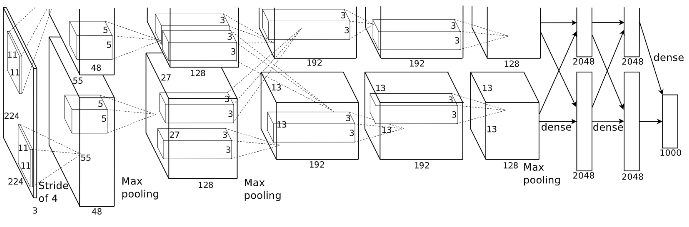
\includegraphics[width=\textwidth]{Images/CNNArchitectures/AlexNet.png}
	\decoRule
	\caption[AlexNet architecture]{AlexNet architecture}
	\label{fig:AlexNet}
\end{figure}

Since AlexNet, most, if not all, CNNs are at least as deep, to achieve high learning capacity and accuracy.

Nowadays, AlexNet is one of the most well-known CNNs and is often used as a benchmark for various hardware solutions, due to its high complexity and number of parameters needed. In total, it uses more than 61 million parameters, which results in a size of about 250MB.

\subsection{ZFNet}
ZFNet \cite{Visualizing-and-Understanding-Convolutional-Networks} (Figure \ref{fig:ZFNet}) is a fine-tuned version of AlexNet by Matthew Zeiler and Rob Fergus, which won the ILSVRC 2013, achieving a top-5 error rate of 14.8\%.

\begin{figure} [H]
	\centering
	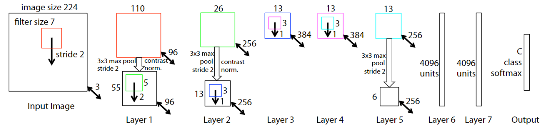
\includegraphics[width=\textwidth]{Images/CNNArchitectures/ZFNet.png}
	\decoRule
	\caption[ZFNet architecture]{ZFNet architecture}
	\label{fig:ZFNet}
\end{figure}

\subsection{GoogLeNet / Inception}
GoogLeNet \cite{Going-Deeper-with-Convolutions} (Figure \ref{fig:GoogLeNet}), also known as Inception v1, designed by Google, won the ILSVRC 2014 with a top-5 error rate of 6.67\%. Provided that GoogLe\-Net's top-5 error rate was near to the human level, organizers had to evaluate these results with the help of a human expert, previously trained for a few days, who achieved a top-5 error rate of 5.1\% for a single model and 3.6\% for the ensemble. This architecture, inspired by LeNet-5, consists of 22 layers but reduces the number of parameters compared to AlexNet from 61 million to only 4 million. The parameter reduction was achieved by using a special module called Inception, which is based on several very small convolutions. To further improve the accuracy, techniques such as batch normalization, image distortions, and RMSProp were used. Note that the auxiliary classifiers, Softmax0 and Softmax1, are only used during the training phase to combat the vanishing gradient problem and to provide regularization.

\begin{figure} [H]
	\centering
	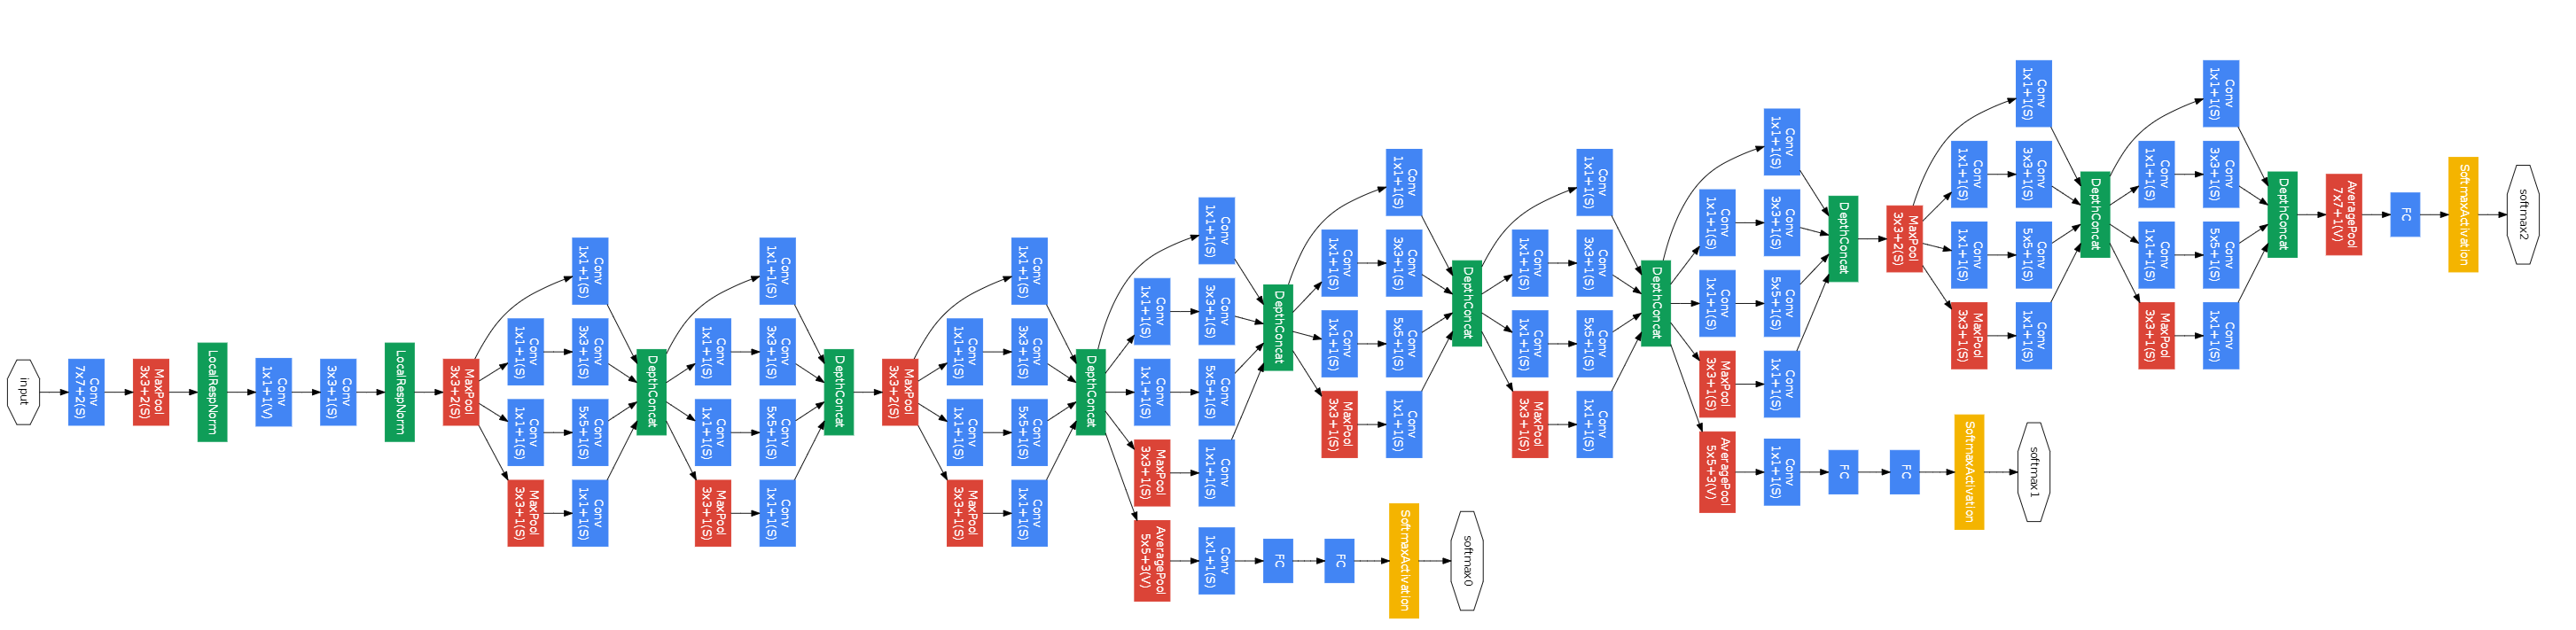
\includegraphics[width=\textwidth]{Images/CNNArchitectures/GoogLeNet.png}
	\decoRule
	\caption[GoogLeNet/Inception v1 architecture]{GoogLeNet/Inception v1 architecture}
	\label{fig:GoogLeNet}
\end{figure}

\subsection{VGGNet}
VGGNet \cite{Very-Deep-Convolutional-Networks-for-Large-Scale-Image-Recognition} (Figure \ref{fig:VGGNet}), designed by Simonyan and Zisserman, was the runner-up ate the ILSVRC 2014. The original architecture consists of 16 layers, but there are other variants with more or fewer layers. In comparison to AlexNet, it uses more filters, and it was trained with 4 GPUs for up to 3 weeks. Nowadays, it is the most preferred network for image feature extraction; however, it can be very challenging, due to its 138 million parameters.

\begin{figure} [H]
	\centering
	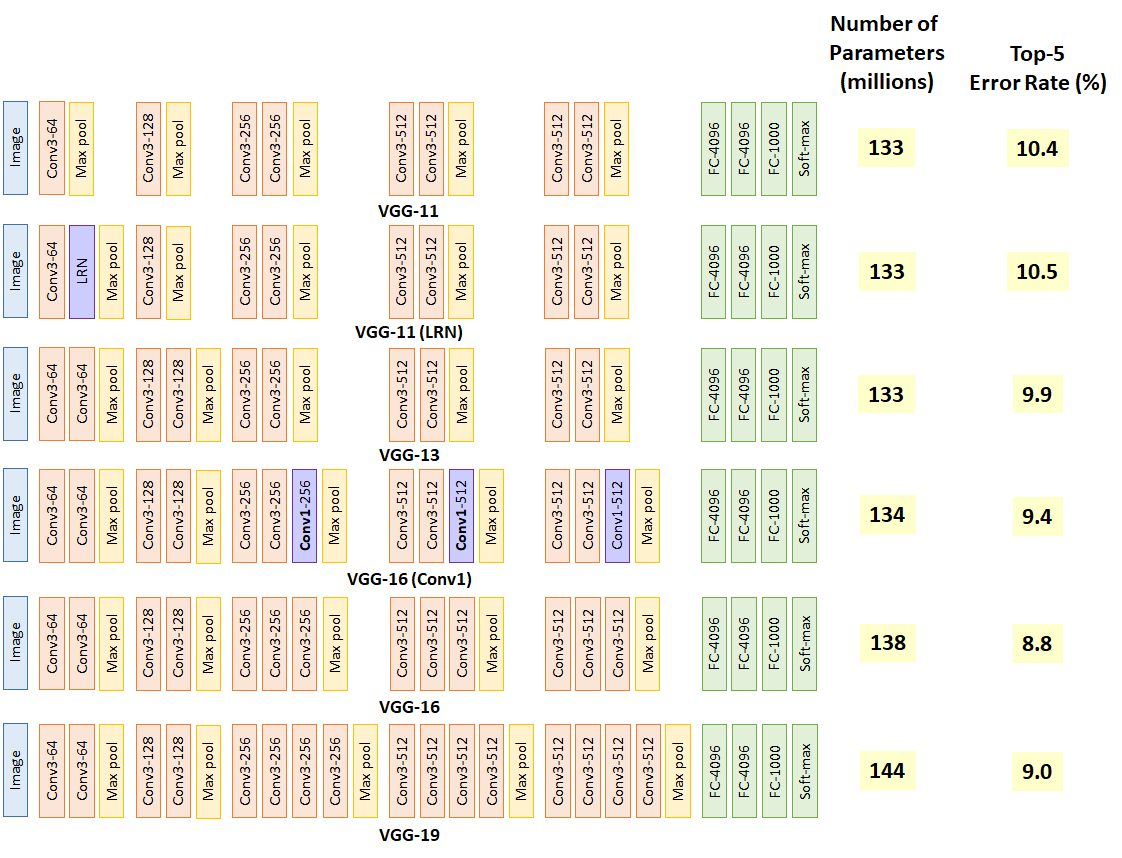
\includegraphics[width=\textwidth]{Images/CNNArchitectures/VGGNet.png}
	\decoRule
	\caption[VGGNet architectures]{VGGNet architectures: \href{https://medium.com/coinmonks/paper-review-of-vggnet-1st-runner-up-of-ilsvlc-2014-image-classification-d02355543a11}{URL}}
	\label{fig:VGGNet}
\end{figure}

\subsection{ResNet}
ResNet \cite{Deep-Residual-Learning-for-Image-Recognition} (Figure \ref{fig:ResNet}), designed by Microsoft, won the ILSVRC 2015 with an outstanding top-5 error rate of 3.57\%, beating the human-level performance. This was achieved with the use of 152 layers. Although the layers' number may be high, its complexity is kept lower than the VGGNet due to its architecture called Residual Neural Network. It uses gated (recurrent) units, a module inspired by the recent successful elements used in RNNs, which, in a sense, skips connections. In addition, heavy batch normalizations are also used.

\begin{figure} [H]
	\centering
	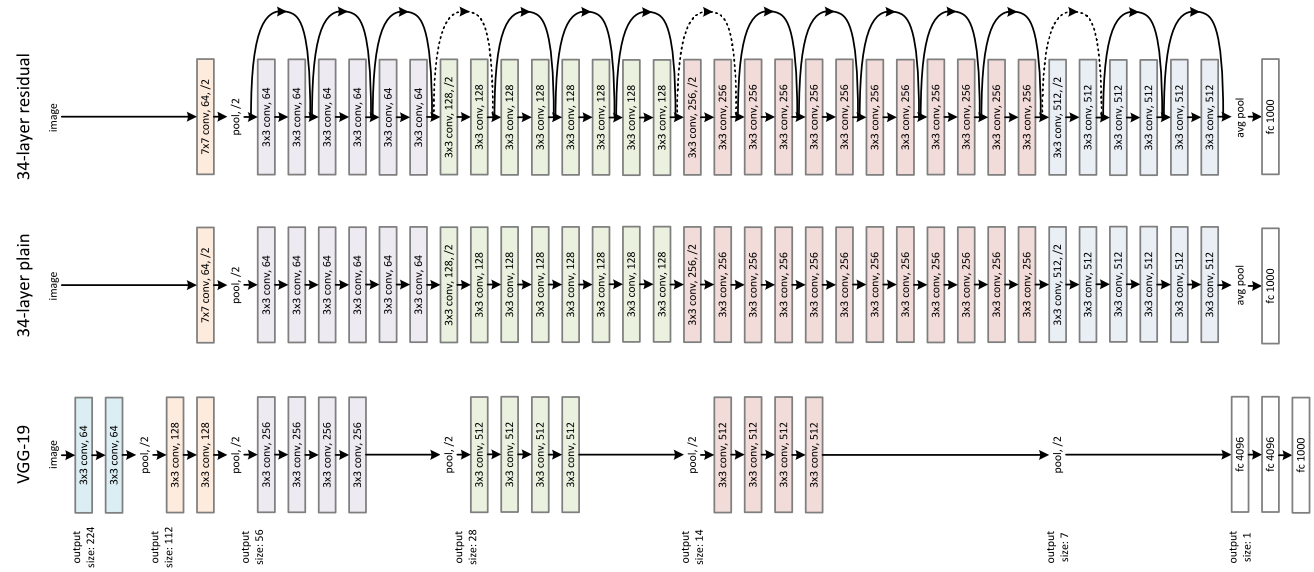
\includegraphics[width=\textwidth]{Images/CNNArchitectures/ResNet.png}
	\decoRule
	\caption[ResNet architecture]{ResNet architecture - Left: the VGG-19 model (19.6 GFLOPs) as a reference. Middle: a plain network with 34 parameter layers (3.6 GFLOPs). Right: a residual network with 34 parameter layers (3.6 GFLOPs). The dotted shortcuts increase dimensions.}
	\label{fig:ResNet}
\end{figure}

\subsection{Summary}
One can observe that all the aforementioned architectures use the same types of layers found on classical CNNs. They only differ in some training techniques, their depths, and hyperparameters. In this work, AlexNet is the primary benchmark used to test the various hardware architectures, because of its simplicity and its high complexity.

\section{Deep Learning Software Frameworks}
There are many software frameworks available for developers to use for their deep learning applications. Their differences, apart from their syntax, are found on the amount of abstraction, portability, and their environment. Some of the most popular ones are described below.

\subsection{Keras}
Keras \cite{Keras-Official-site} \cite{Keras-Wikipedia} is a high-level library for Python, built on top of other lower-level frameworks such as TensorFlow, Theano and CNTK. While the high-level approach reduces the creation of massive deep learning models to single-line functions, it also makes the library's environment less configurable. It is best suited for learning and prototyping, with the abstraction of the mathematical operations applied.

\subsection{CAFFE}
CAFFE (Convolutional Architecture for Fast Feature Embedding) \cite{Caffe-Convolutional-Architecture-for-Fast-Feature-Embedding} \cite{Caffe-Official-site} \cite{Caffe-Wikipedia} is a deep learning framework written in C++, with a Python interface, originally developed at University of California, Berkley. It supports CNN, RCNN, LSTM, and Fully-Connected neural network models, with both CPU and GPU acceleration. Its successor, CAFFE2, also supports RNNs. CAFFE2 is now merged into PyTorch.

\subsection{PyTorch}
PyTorch \cite{PyTorch-Official-site} \cite{PyTorch-Wikipedia} developed by Facebook, is a lower-level framework based on Torch, which supports any kind of neural networks. It contains many pre-trained models, most of those in section \ref{section:CNN-Architectures}, and can also utilize GPU acceleration. It operates with a dynamically updated graph, which allows for changes to the architecture in the process. It is best suited for small projects, prototyping, and research purposes.

\subsection{TensorFlow}
TensorFlow \cite{TensorFlow-Large-Scale-Machine-Learning-on-Heterogeneous-Distributed-Systems} \cite{TensorFlow-Official-site} \cite{TensorFlow-Wikipedia} is the most popular deep learning framework nowadays. Developed by Google, it has interfaces for Python, Javascript, C++, C\#, Java, Go, and Julia. It is the most used framework for production, with support of CPU, GPU, and TPU acceleration. It can, not only, run on powerful computing clusters, but also, on mobile platforms and embedded systems. While it is a lower-level framework and needs much coding, it provides high configurability. In contrast to PyTorch, it operates with a static computation graph, which enhances its efficiency but sacrifices the ease of model modifications; for every modification, a model retrain is needed.

\section{Hardware Solutions}
The most considerable portion of the computation needed in CNNs comes from the Multiply-Accumulate (MAC) operations on floating-point numbers. Usually, networks are trained on GPUs, because they can fulfill the high parallelism needs. For even more exceptional performance on training, TPUs can be used. However, the training phase is considered, most of the time, to be a one-time procedure. Hence, the research community is more focused on accelerating the inference phase. While being a much less computationally intensive procedure compared to training, the inference phase can still be intensive enough to be able to achieve real-time or even faster applications.

Neural networks' inference can be run on CPUs, GPUs, ASICs such as the TPU, and also FPGAs. A brief description of each platform's advantages and limitations is given below.

\subsection{CPUs}
CPUs are multi-purpose processors that can be very flexible in the types of operations they can execute while being very easy to program. They can also execute Single Instruction Multiple Data (SIMD) instructions using the Advanced Vector Extensions (AVX) \cite{AVX-Wikipedia} and Streaming SIMD Extensions (SSE) \cite{SSE-Wikipedia}, and utilize multiple cores. Even though CPUs run at clock speeds in the gigahertz range, they lack the vast amount of computation power compared to other solutions, and they can have high power consumption.

\subsection{GPUs}
Most of the aforementioned deep learning frameworks support GPU acceleration. GPUs can have hundreds or even thousands of more cores compared to CPUs, with even specialized ones called Tensor cores for tensor operations, which makes them ideal for executing algorithms with high parallelism characteristics, such as those used in deep learning. Vector processing creates the bulk of the GPUs' compute power with which the same operation is applied to a large amount of data at the same time. This is achieved by using many Streaming Multiprocessors (SMs) on a single GPU die, which are vector processors that can process up to thousands of operations in a single clock cycle. In addition, due to the massive amounts of data that deep learning algorithms need to handle, High Bandwidth Memory (HBM) can be a perfect fit providing up to 750 GB/s compared to only 50 GB/s offered by traditional CPUs. Moreover, multiple GPUs in a single system can be utilized to further expand its parallelism capabilities.

As of right now, only NVIDIA GPUs are widely supported by most frameworks. NVIDIA's GPUs are optimized for deep learning frameworks with compatibility for Compute Unified Device Architecture Software Development Kit (CUDA SDK) \cite{NVIDIA-CUDA}, which supports many programming languages such as C and C++, increasing the GPUs usability. NVIDIA has also developed the CUDA Deep Neural Network library (cuDNN) \cite{cuDNN-Efficient-Primitives-for-Deep-Learning} \cite{NVIDIA-cuDNN}, designed to accelerate frameworks such as TensorFlow and PyTorch by providing highly-optimized implementations of routines like forward and backward convolution. Furthermore, NVIDIA's TensorRT \cite{NVIDIA-TensorRT} is an SDK for high\-ly optimized inference applications, delivering low latency and high throughput (compared to CPUs). PyTorch also supports PyCUDA \cite{NVIDIA-PyCUDA}, NVIDIA's CUDA parallel computation API for Python.

Although GPUs provide very high performance and throughput, they can be very power inefficient and can introduce high latency per result relative to other solutions.

\subsection{Tensor Processing Units (TPU)}
Tensor Processing Unit (TPU) \cite{In-Datacenter-Performance-Analysis-of-a-Tensor-Processing-Unit} is a custom Application Specific Integrated Circuit (ASIC) that accelerates the inference phase on neural networks designed by Google to improve cost-performance over GPUs. It is deployed to their datacenters since 2015 to accelerate 95\% of their AI needs, and since 2017 Google made its TPU infrastructure available to the public on its Google Compute Engine. The first architecture generation achieves up to 200x speedup compared to a server-class Intel Haswell CPU and up to 70x speedup compared to an NVIDIA K80 GPU. Nowadays, they have designed another two generations of its TPU (latest is TPU v3), and an edge computing solution called Coral Edge TPU \cite{Coral-Edge-TPU}, which comes in various form factors, achieving up to 4 TOPS using only 2 Watts. The first generation of TPUs was targeted for inference applications and was designed for high volume of as low as 8-bit precision computation. However, from the second generation, TPUs support floating-point arithmetic making them ideal for training accelerators.

Each TPU core provides 2 Matrix Multiplier Units (MXUs) and is provided 16GB of HBM (TPUv3) (Figure \ref{fig:tpu-v1-block-diagram}). Each MXU is capable of 16k Multiply-Accumulate (MAC) operation per cycle, which gives the bulk of the compute power. In contrast to GPUs which operate on vector data, TPUs operate on matrices providing up to hundreds of thousands of operations in a single clock cycle. MXU's architecture (Figure \ref{fig:tpu-mxu}) is based on systolic arrays to implement such a large-scale matrix processor. Its systolic mechanism contains a matrix of 256x256 8-bit Arithmetic Logic Units (ALUs) that multiply-and-add 65536 integers per clock cycle, and because TPUs run at 700MHz, they yield performance of 92 TeraOPs per second each. The systolic array chains multiple ALUs, to use the previous ALU's result, and reuse inputs by forwarding them to the next ALUs. In this manner, communication with off-chip memory is significantly reduced \cite{An-in-depth-look-at-Google-first-TPU}.

\begin{figure} [H]
	\centering
	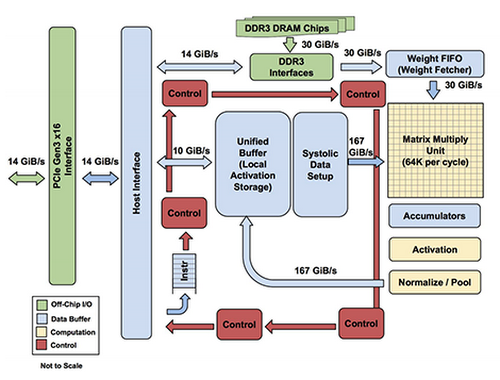
\includegraphics[width=\textwidth]{Images/Hardware/tpu-v1-block-diagram.png}
	\decoRule
	\caption[Google Cloud TPU v1 Architecture Block Diagram]{Google Cloud TPU v1 Architecture Block Diagram: \href{https://cloud.google.com/blog/products/gcp/an-in-depth-look-at-googles-first-tensor-processing-unit-tpu}{URL}}
	\label{fig:tpu-v1-block-diagram}
\end{figure}

\begin{figure} [H]
	\centering
	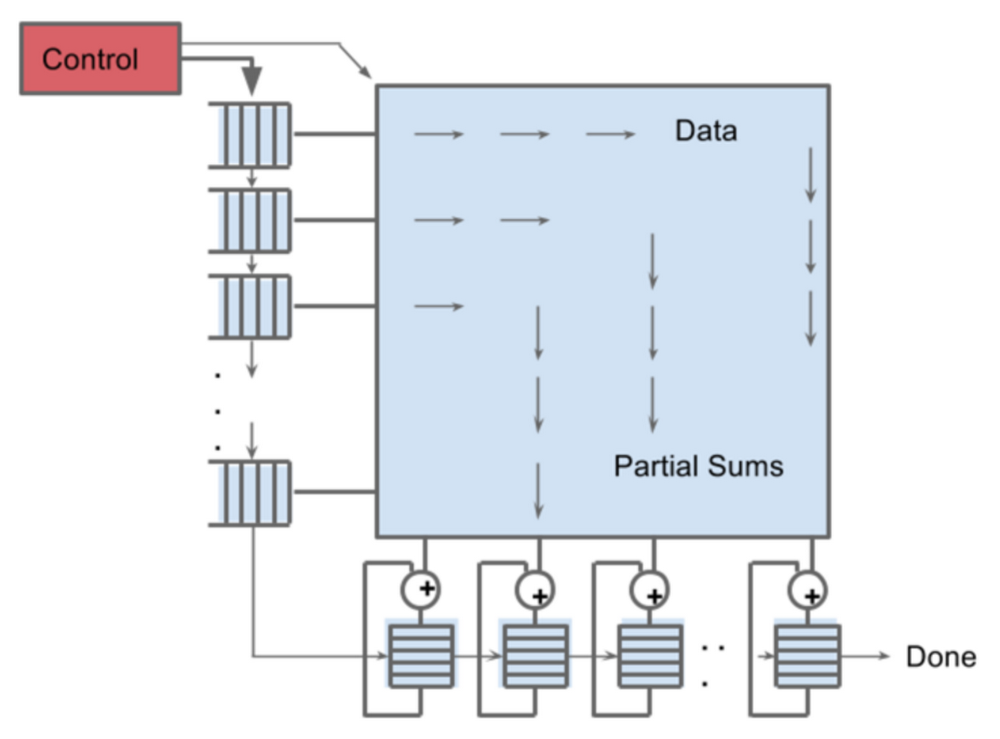
\includegraphics[scale=0.25]{Images/Hardware/tpu-mxu.png}
	\decoRule
	\caption[Google Cloud TPU Matrix Multiplier Unit (MXU)]{Google Cloud TPU Matrix Multiplier Unit (MXU): \href{https://cloud.google.com/blog/products/gcp/an-in-depth-look-at-googles-first-tensor-processing-unit-tpu}{URL}}
	\label{fig:tpu-mxu}
\end{figure}

Every TPU v3 board is comprised of 4 chips (Figure \ref{fig:google-tpu-motherboard}), with each chip containing 2 TPU cores. TPU boards are organized into pods (Figure \ref{fig:tpu-v3-pods}), with each pod containing up to 2048 TPU cores and 32TB total memory \cite{Google-Cloud-TPU}, providing a total of up to 92 PetaFLOPS of performance \cite{Tensor-Processing-Unit-Wikipedia}.

\begin{figure} [H]
	\centering
	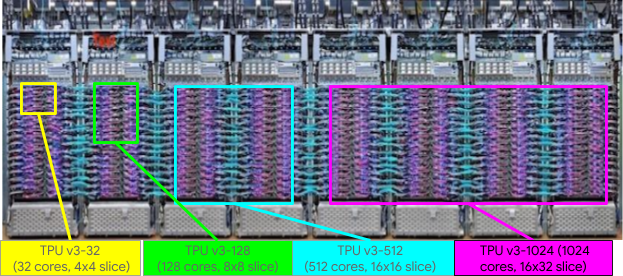
\includegraphics[width=\textwidth]{Images/Hardware/tpu-v3-pods.png}
	\decoRule
	\caption[Google Cloud TPU v3 Pods]{Google Cloud TPU v3 Pods: \href{https://cloud.google.com/tpu/docs/system-architecture}{URL}}
	\label{fig:tpu-v3-pods}
\end{figure}

The TensorFlow framework is used to run applications on TPUs, with a reduced bfloat16 precision. Google created the bfloat16 16-bit floating-point representation standard to provide better training and model accuracy compared to IEEE half-precision representation.

In general, TPUs are worth using with very large models, needing weeks or even months of training, dominated by matrix computations, and no custom TensorFlow operations inside the main training loop. Otherwise, GPUs or ever CPUs may be more suitable and cost-effective \cite{Cloud-Tensor-Processing-Units}.

ASICs, like Google's TPUs, are very costly to design and produce. While they provide the best performance and efficiency, they can become deprecated fast, due to the speed the AI field is developing.

\subsection{FPGAs}
FPGAs provide high flexibility in terms of hardware architectures, unlike all other hardware solutions that are limited to their fixed architecture. For every application, a custom design is developed to provide the computation units in types and volume needed. Computation units are then placed on the so-called FPGA fabric, the programmable part of the chip, to create systems that accelerate specific applications.

Often FPGAs integrate numerous Digital Signal Processing (DSP) blocks, which are hardware elements into the FPGA fabric. DSPs provide optimized hardware for various common mathematical operations such as multiply-accumulate (MAC) and division for representations from floating-point to fixed-point or even integer. DSPs can also be configured as Double-Pumped, allowing them to be clocked at twice the core clock.

Moreover, FPGAs can come with hard processor cores in the same chip that can be used for communication, scheduling, and data pre and post-processing. Such configurations are typically called Multi-Processor System on Chip (MPSoC). FPGAs are a perfect match for fields that come with rapid pace of development, such as AI and ML. Furthermore, they provide high energy efficiency and low latency per result due to the design being specific to the application.

Although FPGAs have Block RAM (BRAM) and some even Ultra RAM (URAM), which is a high-speed type of memory inside the FPGA fabric, they can be bottlenecked due to its limited size. Hence, FPGAs are often provided with big DRAM modules. However, compared to GPUs', which are provided with HBM, FPGAs may still face bandwidth limitations. Such limitations can be overcome the same way ASICs do; by reducing data precision. Reducing data precision is accomplished by converting them from floating-point to lower bitwidth numeric representations, such as half-precision floating point and fixed point. It can also be achieved by data reuse or quantization.

\section{Quantization}
In order to compete with GPUs, FPGAs and TPUs have to minimize their memory bandwidth needs. One of the most effective ways to tackle this problem is by reducing the parameters' memory footprint. This process is called quantization, and it is comprised of various techniques. While, quantization is applied independently of the framework that trains the network and the hardware that runs its inference, the techniques to be used are selected explicitly to the network's environment for best performance optimization.

\textcolor{red}{
Todo: add more details on techniques and reference papers
}

\section{The FPGA Perspective}
While FPGAs can provide significant advantages over other hardware platforms, as of right now, there is no software framework, like TensorFlow and PyTorch, that natively supports FPGA acceleration. Hence, third party architectures have to be used.

\subsection{Xilinx CHaiDNN}
The CHaiDNN \cite{CHaiDNN-GitHub} is an open-source Deep Neural Network inference accelerator library developed by Xilinx for its Ultrascale+ MPSoC devices, mainly focusing on Convolutional Neural Networks. It was initially released in February 2018, with its second version been released in June 2018.

The CHaiDNN is designed for maximum compute efficiency at 6-bit fixed-point data type for both parameters and activations, while also supporting 8-bit fixed-point representations. The data precision can vary even throughout the layers, claiming that a well-crafted data precision combination can result in accuracy similar to a floating-point single precision model. To avoid retraining the network with 6-bit or 8-bit fixed-point representations, Xilinx has developed two quantization techniques, the Dynamic fixed-point quantization, and the Xilinx Quantizer, which are both supported by the CHaiDNN.

Moreover, the CHaiDNN provides configurations that can utilize from 128 up to 1024 Double-Pumped DSPs, with some designs achieving up to 700MHz. For smaller MPSoCs, there is the DietCHai, a miniature version of CHai. URAM is also supported.

Even though the most commonly used layers in various image classification and object detection neural networks are supported, unsupported layers can also be added as software layers and run the network's inference. For performance optimization, some layers, such as the Fully-Connected and Softmax, are implemented as software layers. However, software layers can decrease the inference throughput based on their latencies. In order to tackle this problem, hardware and software layers can be run in parallel, hiding each others' latencies.

To run the inference using the accelerator, PetaLinux has to be running on the MPSoC to handle all the layer job scheduling across all CPU cores and hardware IPs. Network configuration and parameters are given using the Caffe framework's standard (.prototxt, .caffemodel, and mean files).

\subsection{Xilinx Deep Learning Processing Unit (DPU)}
Xilinx Deep Learning Processing Unit (DPU) \cite{PG338-Zynq-DPU-IP-Product-Guide} is a configurable Convolutional Neural Network 8-bit integer inference accelerator developed by Xilinx for its Zynq-7000 SoCs and Zynq Ultrascale+ MPSoCs. It supports most CNNs and can be configured appropriately according to parallelism needs and resource constraints. It was initially released in February 2019, with its latest version 3.2 been released in March 2020.

The DPU IP is implemented in the Programmable Logic (PL) part with direct connections to the Processing System (PS). Instructions are sent from the program running on the Application Processing Unit (APU) to the corresponding DPU core with memory addresses of input images, temporary, and output data. The system's architecture is shown in Figure \ref{fig:dpu-top-block-diagram} (Left) with the APU, High Speed Data Tube, and DPU part all being in the same MPSoC, and RAM being the external Random Access Memory. A more detailed hardware architecture is shown on Figure \ref{fig:dpu-top-block-diagram} (Right). It is worth noting that the on-chip memory is utilized as a buffer for input, temporary and output data, increasing throughput, and efficiency by reusing as much data as possible and reducing external memory communication. The Hybrid Computing Array (Left) or Computing Engine (Right) is comprised of Processing Elements (PEs), creating a deep pipelined design. A PE is based on the fine-grained building blocks found in Xilinx devices, such as multipliers, adders, and accumulators.

\begin{figure} [H]
	\centering
	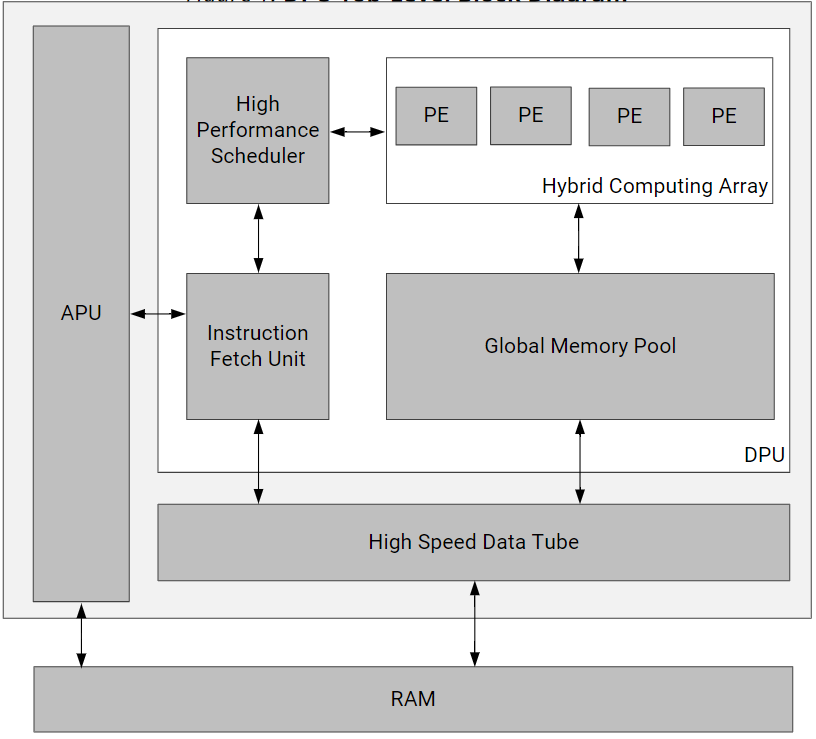
\includegraphics[scale=0.35]{Images/Hardware/dpu-top-block-diagram.png}
	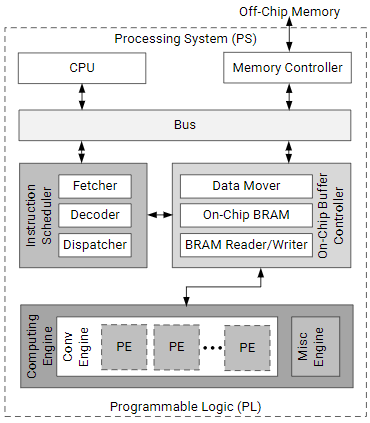
\includegraphics[scale=0.6]{Images/Hardware/dpu-hardware-architecture.png}
	\decoRule
	\caption[Xilinx DPU Architecture]{Xilinx DPU Architecture: Left top-level block diagram, Right hardware architecture: \href{https://www.xilinx.com/support/documentation/ip_documentation/dpu/v3_2/pg338-dpu.pdf}{URL}}
	\label{fig:dpu-top-block-diagram}
\end{figure}

DPU-V1, previously known as xDNN, uses a 96x16 DSP Systolic Array as its main compute unit (Figure \ref{fig:dpu-v1-architecture}). DPU-V2 uses a Hybrid Computing Array (Figure \ref{fig:dpu-v2-architecture}), and DPU-V3E uses multiple instances of Batch Engines in each DPU core (Figure \ref{fig:dpu-v3-architecture}).

\begin{figure} [H]
	\centering
	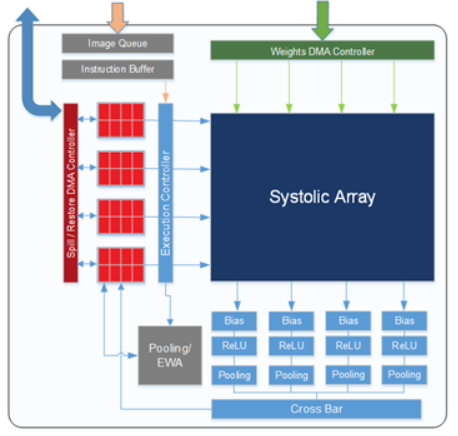
\includegraphics[scale=0.6]{Images/Hardware/dpu-v1-architecture.png}
	\decoRule
	\caption[Xilinx DPU-V1 Architecture]{Xilinx DPU-V1 Architecture: \href{https://www.xilinx.com/html_docs/vitis_ai/1_1/zlx1571919192500.html}{URL}}
	\label{fig:dpu-v1-architecture}
\end{figure}

\begin{figure} [H]
	\centering
	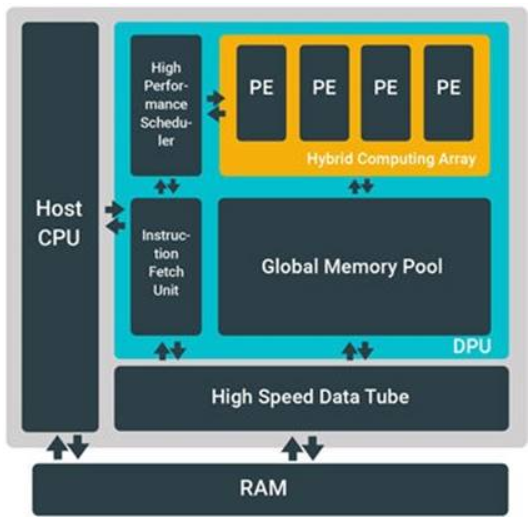
\includegraphics[scale=0.6]{Images/Hardware/dpu-v2-architecture.png}
	\decoRule
	\caption[Xilinx DPU-V2 Architecture]{Xilinx DPU-V2 Architecture: \href{https://www.xilinx.com/html_docs/vitis_ai/1_1/vpt1571919210634.html}{URL}}
	\label{fig:dpu-v2-architecture}
\end{figure}

\begin{figure} [H]
	\centering
	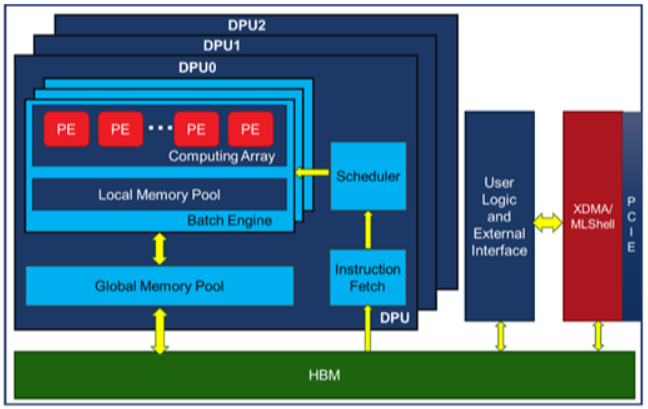
\includegraphics[scale=0.6]{Images/Hardware/dpu-v3-architecture.png}
	\decoRule
	\caption[Xilinx DPU-V3 Architecture]{Xilinx DPU-V3 Architecture: \href{https://www.xilinx.com/html_docs/vitis_ai/1_1/xyt1583919665886.html}{URL}}
	\label{fig:dpu-v3-architecture}
\end{figure}

In contrast with the CHaiDNN, all layers, including the Fully-Connected and Softmax layers, are hardware accelerated. Currently, implementing up to four DPU cores in a single DPU IP is supported, and there is an option of using Double Data Rate DSPs (Double-Pumped DSPs). Furthermore, there are architectures for various parallelism needs, starting from 512 operations per cycle per core up to 4096 operations per cycle per core.

The Xilinx Vitis AI development environment \cite{Xilinx-Vitis-AI}, released in December 2019, is Xilinx's development platform for AI inference applications using its hardware platforms, which provides optimized IPs, tools, and libraries including the aforementioned Xilinx DPU. The Xilinx Vitis AI stack (Figure \ref{fig:vitis-ai-stack}) has to be used to run a network's inference using the DPU accelerator. The network's program giving instructions and orchestrating the data transfers has to run on top of PetaLinux. This program is generated with substantial instruction optimizations using the Xilinx Vitis AI compiler. This program has to be regenerated with every network or hardware configuration change. The network's quantization is done using the Xilinx Vitis AI Quantizer, generating the appropriate 8-bit integer parameters.

\begin{figure} [H]
	\centering
	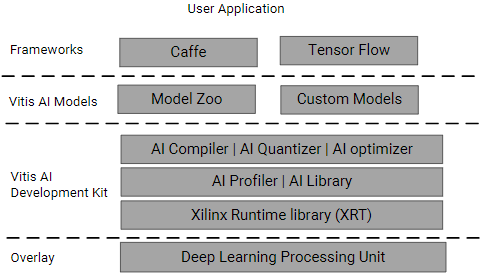
\includegraphics[scale=0.6]{Images/Hardware/vitis-ai-stack.png}
	\decoRule
	\caption[Xilinx Vitis AI Stack]{Xilinx Vitis AI Stack: \href{https://www.xilinx.com/support/documentation/ip_documentation/dpu/v3_2/pg338-dpu.pdf}{URL}}
	\label{fig:vitis-ai-stack}
\end{figure}

\subsection{NVIDIA NVDLA}
NVIDIA's Deep Learning Accelerator (NVDLA) \cite{NVIDIA-NVDLA}, initially released in Q3 2017, is a free and open architecture project seeking to standardize the design of deep learning inference accelerators.

There are two main system implementations; the headless and the headed. The headless implementation expects the main system's processor to manage the accelerator, while the headed implementation expects a companion microcontroller, tightly coupled to the NVDLA sub-system, to do the management.

NVDLA is comprised of five components, Convolution core, Single Data processor, Planar Data processor, Channel Data processor, Dedicated Memory, and Data Reshape Engine, which are separate and independently configurable. Each block's input and output data transfers can be performed either in memory-to-memory using the Independent operation mode, or by passing through some internal results to next blocks using the Fused operation mode (Figure \ref{fig:nvdla-hardware-architecture}). Furthermore, NVDLA supports a wide range of data types, from binary and 4-bit integer up to 64-bit floating-point.

\begin{figure} [H]
	\centering
	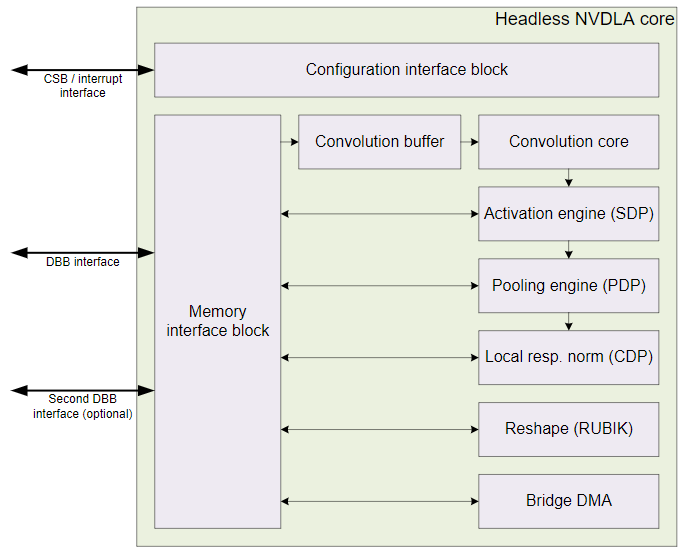
\includegraphics[scale=0.6]{Images/Hardware/nvdla-hardware-architecture.png}
	\decoRule
	\caption[NVIDIA NVDLA Hardware Architecture]{NVIDIA NVDLA Hardware Architecture in Fused operation mode: \href{http://nvdla.org/primer.html}{URL}}
	\label{fig:nvdla-hardware-architecture}
\end{figure}

The convolution core supports sparse weight compression to reduce memory bandwidth, as well as Winograd for computing efficiency for specific kernel sizes. Batch convolution is also supported to reduce memory bandwidth. In addition, a convolution buffer is added as internal RAM to avoid communication with external system memory.

The Single Data Point processor implements the various linear and non-linear activation functions used in CNNs. For the non-linear functions, a lookup table is used, while for the linear functions, a simple bias and scale are used.

The Planar Data processor supports minimum, maximum, and average pooling operations, with kernel sizes configurable during runtime.

The Cross-channel Data processor implements the local response normalization.

The Data Reshape engine performs data format transformations for operations such as slice and reshape-transpose.

In general, NVDLA is a highly customizable and modular architecture, with various configurations suitable for both FPGAs and ASICs.

\section{Thesis Approach}
